\section{What}

\begin{wrapfigure}{R}{0.3\textwidth}
\centering
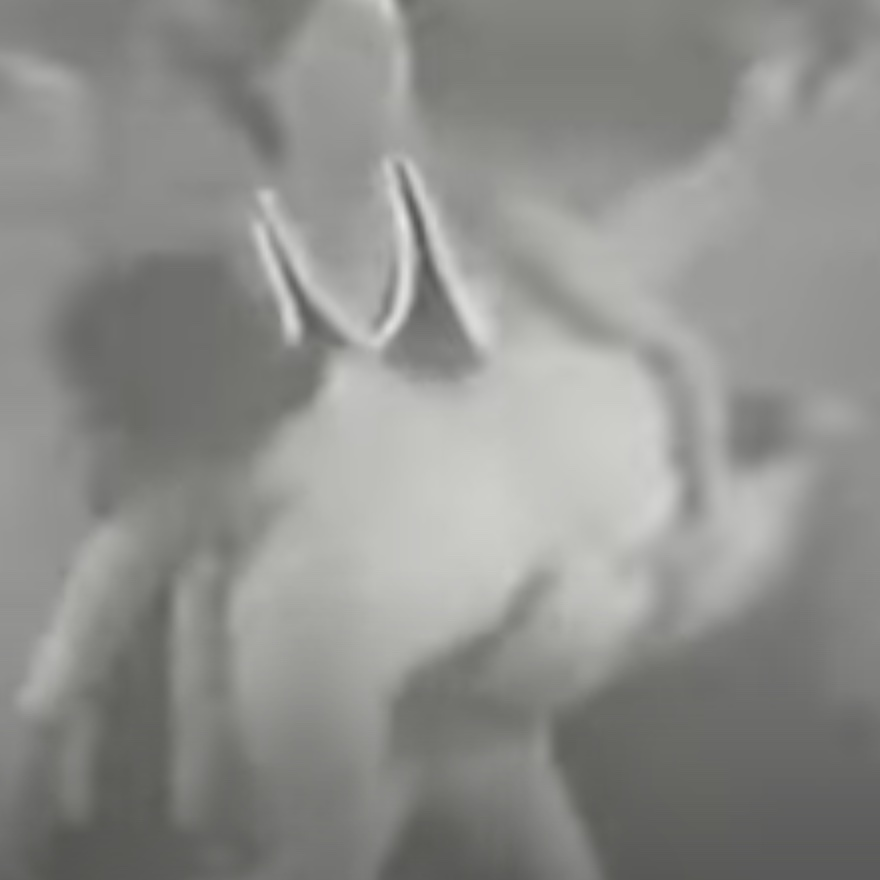
\includegraphics[width=0.25\textwidth]{images/what.jpg}
\end{wrapfigure}

So what is CI? A dance, a sport, acrobatics or martial arts? Well, all of it.

It could be considered a form of improvised partner dancing, a contemporary dance form, an "art-sport". An exploration of one's body in relationship to others by using principles of sharing weight, touch, and movement awareness. To play with the artistry of falling off balance and counterbalance. To learn the mechanics of the body to handle someone's weight or to be lifted, along with breathing techniques. At its core it involves mindfulness, sensing and collecting information.

Emphasize is put on:
\begin{itemize}
	\item \textbf{Experimental dance}: practice-based research in dance laboratories
	\item \textbf{Theatrical form}: improvised performances and lectures-demonstrations
	\item \textbf{Educational tool}: training for professional dancers in improvisation
	\item \textbf{Social dancing}: at informal gatherings called "jams"
	\item \textbf{Awareness practice}: being able to listen to the subtleties in contact
\end{itemize}

This art form is not only for the young and well-trained, as there is no real requirement for acrobatic performance. The body just needs to be mobile and the bones bear some weight.

There is a broad global community, which organizes social dances, so-called "jams", and practitioners often overlap with the ecstatic dance communities.


\subsection{Definitions}

\textbf{Steve Paxton} himself stated in 1979: \textit{The exigencies of the form dictate a mode of movement which is relaxed, constantly aware and prepared, and onflowing. As a basic focus, the dancers remain in physical touch, mutually supportive and innovative, meditating upon the physical laws relating to their masses: gravity, momentum, inertia, and friction. They do not strive to achieve results, but rather, to meet the constantly changing physical reality with appropriate placement and energy.}

\textbf{Nancy Start Smith} once mentioned, it "\textit{resembles other familiar duet forms, such as the embrace, wrestling, surfing, martial arts, and the Jitterbug (Lindy Hop and swing dances), encompassing a wide range of movement from stillness to highly athletic}".

\textbf{Daniel Lepkoff} states about the core of CI, to "\textit{put focus on bodily awareness and physical reflexes, rather than consciously controlled movements. Precedence of body experience first, and mindful cognition second, is an essential distinction between CI and other approaches to dance.}"
